\documentclass[12pt]{article}
\usepackage{hyperref}
\usepackage[fleqn]{amsmath}
\usepackage{amsfonts}
\usepackage{float}
\usepackage{amsthm}
\usepackage{graphicx}


\theoremstyle{remark}
\newtheorem{definition}{Defination}[section]

\title{A Note for Solving String Constraints with Split Function}
\author{Denghang Hu}
\begin{document}
\maketitle

\section{Preliminary}
\subsection{Incremental Nondeterministic Cost Register Automaton (INCRA)}
A \textit{incremental nondeterministic cost register automaton} (INCRA) $\mathcal{A} $ is a tuple $(Q, \Sigma, \delta,q_0,F, R)$ where:
\begin{itemize}
    \item $Q$ is a finite set of \textit{states}.
    \item $\Sigma$ is the alphabet.
    \item $\delta\in Q\times\Sigma\times Q\times M$ is the \textit{transition relation}. $M$ is the set of the update function $\eta$ satisfying that for each $r\in R$, $\eta(r) = r+c$ for some integer constant $c$.
    \item $q_0\in Q$ is the $initial$ state.
    \item $F\subseteq Q$ is the set of $final$ states.
    \item $R = r_1\cdots r_m$ is vector of counters.
\end{itemize}
For a string $w=a_1\cdots a_n $, a run of $\mathcal{A}$ on $w$ is a state sequence $q_0\cdots q_n$ such that for each $i\in[n]$, $(q_{i-1},a_i,q_i,\eta)\in \delta$. A run $q_0\cdots q_n$ on formula $\phi$ is $accepting$ if $q_n \in F$ and $R\models \phi$. INCRA equal to NFA when $R=\emptyset$.
\subsection{Special INCRA for Array}
We define a special INCRA $\mathcal{A}^s$ for \textbf{array} sort. $\mathcal{A}^s$ use a preserved character '$\#$' as $array$ elements separator (note that $\#\not\in\Sigma_{\mathcal{A}^s}$). The speciality of $\mathcal{A}^s$ rely on  its construction.\\
Consider $array$ $A$ with $|A|=m+1$ and assume that for each $i\in\{0,\cdots, m\}$, $A[i]\in \mathcal{A}_i$, then we can construct $A^s=(\bigcup\limits_{0\leq i \leq m} Q_i,\bigcup\limits_{0\leq i \leq m} \Sigma_i, \delta', q_0^{\mathcal{A}_1}, F^{\mathcal{A}_m}, \bigcup\limits_{0\leq i \leq m} R_i), $ as fig \ref{fig:special_nfa}.Note that the language of $A^s$ is $\mathcal{L}(A_1)\cdot\{\#\}\cdot\mathcal{L}(A_2)\ ... \ \cdot\{\#\}\cdot \mathcal{L}(A_{m}) $.
\begin{figure}[H]
    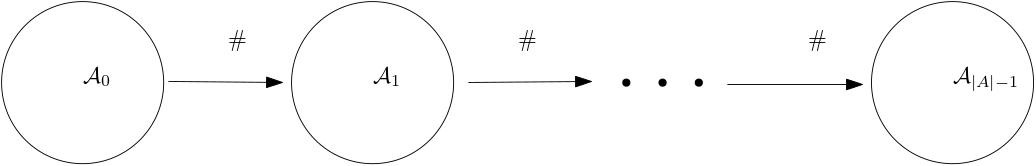
\includegraphics[width=\linewidth]{special_nfa.png}
    \caption{NFA of array $A$}
    \label{fig:special_nfa}
\end{figure}

\section{Straight-Line String Theory with Integer and Array $SL_{I,A,S} $}
We defined a theory $SL_{I,A,S}$ with three sorts: \textbf{string}, \textbf{integer} and \textbf{array}. The \textit{elements} of \textbf{array} can only be \textbf{string} sort. As a convention, the $index$ of \textbf{array} is \textbf{Integer} sort.
\subsection{Syntax}
The syntax of $SL_{I,A,S}$ is defined as fig \ref{fig:syntax}, where $\mathcal{A}$ is an NFA, $\mathcal{A}^s $ is a special NFA for \textbf{array} sort and $\circ \in \{=,\not=, <, \leq, >, \geq \}$. For technical convenience, we assume that all assignments in F are \textit{Static Singly Assignment (SSA)} form.
\begin{figure}[H]
    % denote
    $u,v,\cdots$  \hfill{String constants}\\
    $x,y,\cdots$  \hfill{String varibles}\\
    $m,n,\cdots$  \hfill{Integer constants}\\
    $i,j,\cdots$  \hfill{Integer varibles}\\
    $M,N,\cdots$  \hfill{Array constants}\\
    $X,Y,\cdots$  \hfill{Array varibles}\\ 

    % term and expression
    $s \ ::= \ u \ |\ x$ \hfill{String term}\\
    $t \ ::= \  m \ |\ i \ |\ ct \ |\ t+t \ |\ t-t \ |\ |A| $ \hfill{Integer term}\\
    $A \ ::= \  M \ |\ X  $ \hfill{Array term}\\
    $\beta \ ::= \  m \ |\ |A| \ |\ |A|+m  $  \hfill{Bound expression}\\

    % formula
    $LA \ ::= \ t\circ t \ |\ LA\wedge LA \ |\ \neg LA $  \hfill{Linear arithmatic}\\
    $SC \ ::= \ x=s \ |\ x=A[t] \ |\ x=s\cdot s \ |\ x=\mathrm{join}(A,u) \ |\ s\in\mathcal{A} \ |\ SC\wedge SC $   \flushright{String constraints}\\
    $AC \ ::= \ A = \mathrm{split}(s,e) \ |\ A = A[\beta_1:\beta_2] \ |\ A = A[t\rightarrow s] \ |\ A\in \mathcal{A}^s \ |\ A = \mathcal{T}(A) $ \flushright{Array constraints}\\ 
    $F \ ::= \  LA \ |\ SC \ |\ AC \ |\ F\wedge F $ \hfill{Formula of $SL_{I,A,S} $}
    \caption{Syntax of $SL_{I,A,S}$}
    \label{fig:syntax}
\end{figure}


\subsection{Semantic}
The semantic of $SL_{I,A,S} $ is:
\begin{itemize}
    \item $A[t]$ : Return the $element$ of $A$ at index $t$.
    \item $A[t\rightarrow s]$ : Return a new array the same as $A$ except  that the $element$ of $A$ at index $t$ changes to string $s$.
    \item $s\cdot s$ : String concatenation.
    \item $\mathrm{join}(A,u) $ : Return a new string by concatenating all of $elements$ in array $A$, separated by a specified separator string $u$.
    \item $\mathrm{split}(s,e) $ : Return a new array by dividing string $s$ into ordered substring array. The separator string is regular expression $e$.
    \item $\mathcal{T}(A) $: Return a new array by applying transducer $\mathcal{T}$ on each $element$ of array $A$. 
    \item $A[\beta_1:\beta_2] $ Return a new array which is the subarray of $A$.
\end{itemize}
\subsection{Defination of Straight-Line Restriction }
We consider two sorts: \textbf{string} and \textbf{array}.
\begin{definition}[Relational constraints ]
    Relational constraints $\phi$ are defined by the following rules:
    \begin{align*}
        \phi \ ::= \ x=s\cdot s \ |\ x=\mathrm{join}(A,u) \ |\ A = \mathrm{split}(s,e) \ |\ A = A[\beta_1:\beta_2] \ |\ A = A[t\rightarrow s] \ |\ \phi \wedge \phi
    \end{align*}
\end{definition}
\begin{definition}[Straight-line relational constraints] 
    A relational constraint $\phi$ is straight-line if $\phi = \bigwedge\limits_{1\leq i \leq m} x_i = P_i$ such that
    \begin{itemize}
        \item $x_1,\cdots,x_m $ are mutally distinct.
        \item For each $i\in [m] $, all the varibles in $P_i$ are either source varibles or varibles in set $\{x_1,\cdots,x_{m-1} \}$.
    \end{itemize} 
\end{definition}
\begin{definition}[Straight-line formula]
    A formula $F$ of $SL_{I,A,S}$ is straight-line iff all relational constraints in $F$ are straight-line.
\end{definition}

\section{Pre-image of Assignment}
\subsection{Array Assignment}
Assume $A\in A^s$ and $A^s=(Q, \Sigma, \delta,q_0,F,R)$ construct like fig \ref{fig:special_nfa}.
\begin{itemize}
    \item $A = \mathrm{split}(s,e)$: assume $e\in \mathcal{A}_e$, then we can construct $\mathcal{B}=(Q', \Sigma', \delta',q_0,F,R)$ like fig \ref{fig:pre_image_split} s.t $s\in B$.
    \item $B = A[\beta_1:\beta_2]$:  
\end{itemize}
\begin{figure}
    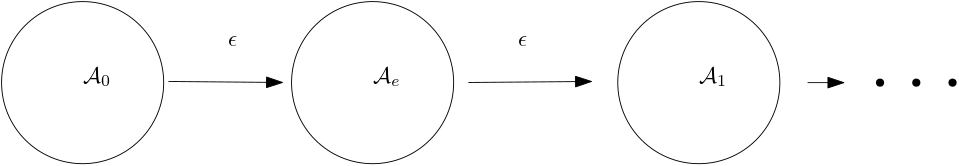
\includegraphics[width=\linewidth]{pre_image_split.png}
    \caption{pre-image of split operation}
    \label{fig:pre_image_split}
\end{figure}
\bibliographystyle{abbrv} % 指定格式,
% \bibliographystyle{apa} % 这是姓名年份应用格式
\bibliography{ref} %  ../.bib表示bib的具体位置
\end{document}